%!TEX program = xelatex
\documentclass{beamer}

\usetheme{metropolis}  % Use metropolis theme

%%
% Configure type font

\usepackage[T1]{fontenc}
\usepackage{newpxtext,eulerpx}

\usepackage{url}

\hypersetup{colorlinks} % Comment this line if you don't wish to have colored links
\usepackage{microtype} % Improves character and word spacing


\usepackage{texnames}
\usepackage{amsmath,amsfonts,amssymb,amsthm}
\usepackage{bm,bbm}
\usepackage[]{subfig}
\usepackage{siunitx}


\usepackage{graphicx} % Needed to insert images into the document
\graphicspath{{./Figures/}} % Sets the default location of pictures
\setkeys{Gin}{width=\linewidth,totalheight=\textheight,keepaspectratio} % Improves figure scaling

\newcommand{\E}{\operatorname{E}}
\newcommand{\Var}{\operatorname{Var}}
\newcommand{\CV}{\operatorname{CV}}

\usepackage{xspace} % Used for printing a trailing space better than using a tilde (~) using the \xspace command

\newcommand{\monthyear}{\ifcase\month\or January\or February\or March\or April\or May\or June\or July\or August\or September\or October\or November\or December\fi\space\number\year} % A command to print the current month and year

\setcounter{secnumdepth}{2}
\setcounter{tocdepth}{2}

\newcommand{\blankpage}{\newpage\hbox{}\thispagestyle{empty}\newpage} % Command to insert a blank page

%%
% Configure math typesetting
\usefonttheme{professionalfonts}  % required for mathspec
\usepackage{mathspec}

%%
% Configure colors
\setbeamercolor{frametitle}{bg=normal text.bg, fg=normal text.fg}

%%
% Configure title graphic positioning
\setbeamertemplate{title graphic}{%
  \vbox to 0pt {
    \vspace*{.75\textheight}  % change the value as necessary
    \hfill\inserttitlegraphic%
  }%
  \nointerlineskip%
}

\title{Operational Statistics for SAR Imagery}
\subtitle{A hands-on autumn course}
\date{September 2019}
\author{Alejandro C.\ Frery}
\institute{%
Laborat\'orio de Computa\c c\~ao Cient\'ifica e An\'alise Num\'erica\\
Universidade Federal de Alagoas
}

\titlegraphic{\includegraphics[width=2.5cm]{laccan.pdf}}

\mode<article>{\lecturenumber{1}}

\begin{document}

\maketitle

\mode*  % ignore text outside frame in presentation mode

This is your lecture abstract. It should contain a short description of the lecture contents, what its goals are, and preferably not exceed a few dozen words.\marginnote{Do not forget to use margin notes to add more context to your material.}

\begin{frame}{Thanks!}
	This course happens thanks to the kind invitation of Prof.\ Xiangrong Zhang, and to the hospitality of her team.
	
	\centering
	\includegraphics[width=\linewidth]{/Users/acfrery/Documents/Transparencias/Figuras/mcz-gru-doh-hkg-xmn-hnd-pek-xiy.png}
\end{frame}


\section{Introduction}

\begin{frame}{Before we start}
\begin{alertblock}{The course}
{\scriptsize Synthetic Aperture Sensors are a basilar tool in Remote Sensing because of their ability to operate day and night, and under unfavorable atmospheric conditions. Moreover, they provide information about the interaction between the target and microwaves. The physics of such imaging is known to yield data with unique statistical properties. Understanding such features is at the core of SAR Remote Sensing. We will see the basic models for these data, along with estimators and their properties. The focus will be in both analytic and graphical tools. We will use the R platform, which has excellent numerical properties and is well-suited for the task of extracting information from the data. Among the topics to be covered are the multiplicative model (Gamma, G, G0 and K distributions), estimation by analogy and maximum likelihood, model checking, data visualization, comparison of estimators, contamination, and classification. All participants are required to use a computer with a connection to the Internet, R, and RStudio (\textit{Free/Libre Open Source Software}).}
\end{alertblock}
\end{frame}

\begin{frame}{What are we supposed to learn in this course?}
Although the application and \textit{leitmotif} is SAR image analysis, the most important message can be split in the following topics:
\begin{itemize}
\item The importance of \textbf{understanding} the problem at hand
\item Which are the basic underlying hypothesis of the processes that turn into the \textbf{data} I have?
\item What can I know about the \textbf{models} I will be dealing with?
\item How can I turn such knowledge into \textbf{tools}?
\item How can I use these tools to extract \textbf{information}?
\item How can I \textbf{communicate} this information?
\end{itemize}
\end{frame}

\begin{frame}{Basic knowledge and tools}

\begin{alertblock}{Concepts}
\begin{itemize}
\item Elements of Probability: distribution, expected value, Central Limit Theorem
\item Elements of Statistics: sample, inference, tests
\item Elements of Programming
\end{itemize}
\end{alertblock}

\begin{alertblock}{Tools}
\begin{itemize}
\item Github and \LaTeX (if you want to have access to the book, code and data)
\item \texttt R and \texttt{RStudio}
\end{itemize}
\end{alertblock}
\end{frame}

\begin{frame}{Evaluation}
I will give assignments during the course, and I expect you to produce a report in \LaTeX, with references managed with \BibTeX, and code in \texttt R for the plots and analyses.

The report will be made available through Git, for instance Github or Bitbucket.
\end{frame}

\begin{frame}{Before we start\dots\ really}
Let's make this more a conversation than a course.

I need you to participate!

acfrery@laccan.ufal.br\\
WeChat ID: \texttt{alex0x0x0x} (naught, not ``o'')
\end{frame}

\section{SAR Sensors}

\begin{frame}{What is SAR?}
	\centering
	\includegraphics[width=.99\linewidth]{/Users/acfrery/Documents/Transparencias/Figuras/bat}
\end{frame}

\begin{frame}
	\frametitle{Basic Characteristics}
	%
	\begin{itemize}%[<+-| alert@+>]
		
		\item Synthetic Aperture Radar (SAR) and Polarimetric SAR (PolSAR) sensors have been successfully used  in remote sensing.
		\begin{itemize}
			\item data can be captured independently of weather conditions, because the sensor is active, 
			\item they measure mostly geometry and dielectric constant, as they work in the microwaves region of the spectrum,
			\item depending on the sensor and target characteristics, the signal penetrates through soil, canopies etc.
		\end{itemize}
		
		\item SAR and PolSAR systems can provide images with high spacial resolution but contaminated by an interference pattern, called \alert{speckle}. 
		%Figure~\ref{fig:Flevoland} exhibits AIRSAR image of Flevoland (Netherlands).
	\end{itemize}
\end{frame}

\begin{frame}{SAR image over a Landsat image}
	\centering
	\includegraphics[angle=-90,width=\linewidth]{/Users/acfrery/Documents/Transparencias/Figuras/SARSaara.jpg}
\end{frame}

\begin{frame}{SAR Image}
	\centering
	\includegraphics[width=\linewidth]{/Users/acfrery/Documents/Pessoas/AbraaoNascimento/ImgFig/speckle000}
\end{frame}


\section{Intensity SAR Data}

\begin{frame}
Assume we illuminate an area with electromagnetic energy having $N$ elementary backscatterers.
Each backscatterer $i$ will return a fraction of the incident energy $A_i$ with phase $\phi_i$.
The total returned complex signal is, therefore,
\begin{equation}
S = \sum_{i=1}^{N} A_i \exp\{\mathbf j \phi_i\} = 
\underbrace{{\sum_{i=1}^{N} A_i \cos \phi_i}}_{\Re(S)} +\mathbf j \underbrace{ \sum_{i=1}^{N} A_i \sin \phi_i}_{\Im(S)}, 
\label{Eq:ComplexBackscatter}
\end{equation}
where $\mathbf j=\sqrt{-1}$ is the imaginary unit.
This is usually called complex scattering.
Fig.~\ref{Fig:ComplexScattering} illustrates an example with $N=10$ backscatterers (black arrows) and the resulting complex scattering (red arrow).
\end{frame}

\begin{frame}
\begin{figure}
\centering
\includegraphics[angle=-90,width=\linewidth]{Scattering}
\caption{Example of complex scattering with $N=10$ elementary backscatterers}\label{Fig:ComplexScattering}
\end{figure}
\end{frame}

\begin{frame}[allowframebreaks]
We have to make some assumptions in order to have a statistical description of the complex return $S$.
These assumptions stem from the fact that we are using microwaves whose typical wavelength is of the order of centimeters, and spatial resolutions of the order decimeters.
This leads to:
\begin{small}
\begin{itemize}
\item[A1:] we are observing backscatterers whose size is smaller than the wavelength, so $N\to\infty$; think, for instance, of the case of imaging a grass field.
\item[A2:] there is no reason to expect that one or a few of these backscatterers dominate the return of the rest; there is no ``mirror'' in our resolution cell.
\item[A3:] the (non-negative) amplitudes $A_i$ are independent.
\item[A4:] there is no reason to expect any particular organization or phase dominance; with this, we may assume that the phases $\phi_i$ are outcomes of independent identically distributed Uniform random variables with support $(-\pi,\pi]$.
\item[A5:] there is no association between phases and amplitudes.
\end{itemize}
\end{small}
With these hypotheses, and using the Central Limit Theorem,	 it is possible to prove that the real and imaginary parts of $S$ are independent Gaussian random variables with zero mean and the same variance $\sigma^2/2$; $\sigma^2$ is often referred to as backscatter.
Two targets with different backscatter only differ in the variance of their complex return $S$.

\end{frame} 

\begin{frame}[allowframebreaks]

More often than not, instead of dealing directly with the complex scattering $S$ one prefers to handle its amplitude $A=|S|$ or intensity $I=|S|^2$.
Without loss of generality, we will prefer the latter.
If the real and imaginary parts of the complex scattering $S$ are independent zero-mean Gaussian random variables with variance $\sigma^2/2$, then the intensity follows an Exponential distribution with mean $\sigma^2$.
\end{frame}

\begin{frame}[allowframebreaks]
A unitary-mean exponential random variable has its distribution characterized by the density
\begin{equation}
f_Z(z) = e^{-z} \mathbbm 1_{(0,\mathbbm R_+)}(z),
\end{equation}
where $\mathbbm 1_{A}(z)$ is the indicator function of the set $A$, i.e., it takes value $1$ inside $A$ and zero otherwise.
Denote this situation $Z\sim E(1)$, and notice that its expected value is $\E(Z)=1$ and its variance is $\Var(Z)=1$.

Being scale-invariant, if $Z'\sim E(1)$, then $Z=\sigma^2 Z'$ has density
\begin{equation}
f_Z(z) = \frac{1}{\sigma^2}e^{-z/\sigma^2} \mathbbm 1_{(0,\mathbbm R_+)}(z),
\end{equation}
and we denote this situation $Z\sim E(\sigma^2)$.
The cumulative distribution function of $Z\sim E(\sigma^2)$ is 
\begin{equation}
F_Z(z) = (1-e^{-z/\sigma^2}) \mathbbm 1_{(0,\mathbbm R_+)}(z).
\end{equation}

The mean and variance of $Z\sim E(\sigma^2)$ are, respectively, $\E(Z)=\sigma^2$ and $\Var(Z) = \sigma^4$.
With this, its coefficient of variation is one: $\CV(Z) = \sqrt{\Var(Z)}/\E(Z) = 1$.

Fig.~\ref{Fig:ExponentialDistribution} shows the densities, cumulative distribution functions and densities in semilogarithmic scale of three Exponential distributions, namely those with means equal to $1/2$, $1$ and $2$.

\begin{figure}[hbt]
\centering
\subfloat[Densities]{\includegraphics[width=.32\linewidth]{ExponentialDensities}}
\subfloat[Cumulative Distribution Functions]{\includegraphics[width=.32\linewidth]{ExponentialCDFs}}
\subfloat[Densities in semilog scale]{\includegraphics[width=.32\linewidth]{ExponentialDensitiesSemilog}}
\caption{Densities, cumulative distribution functions, and densities in semilogarithmic scale of the exponential distribution with means $1/2$, $1$ and $2$ (red, black, blue, resp.)}\label{Fig:ExponentialDistribution}
\end{figure}

The semilogarithmic scale is particularly useful at revealing the tail behavior of distributions: this one is linear.
\end{frame}

\subsection{Multilook processing}
\begin{frame}

Multilook processing is often applied in order to improve the signal-to-noise ratio, which can be measured as the reciprocal of the coefficient of variation.
It consists of using the mean of $L$ independent observations:
\begin{equation}
Z = \frac1L \sum_{\ell=1}^{L} Z_\ell.
\end{equation}
If each $Z_\ell$ follows an exponential distribution with mean $\sigma^2$, we have that $Z$ obeys a Gamma distribution with mean $\sigma^2$ and shape parameter $L$.
This distribution is characterized by the density
\begin{equation}
f_Z(z;L,\sigma^2) = \frac{L^L}{\sigma^{2L}\Gamma(L)} z^{L-1} 
	\exp\big\{ -L z / \sigma^2
	\big\},
	\label{eq:SARGammaDensity}
\end{equation}
where $\Gamma(\nu)$ is the Gamma function given by $\Gamma(\nu)=\int_{\mathbbm R_+} t^{\nu-1} e^{-t} dt$.
We denote this situation $Z\sim\Gamma(\sigma^2,L)$
This is also a scale-invariant distribution, in the sense that if $Z'\sim\Gamma(1,L)$, then $Z=\sigma^2 Z'\sim \Gamma(\sigma^2,L)$.

Fig.~\ref{Fig:GammaDistribution} shows three cases of the Gamma distribution with unitary mean and shape parameters (Looks) equal to $1$ (the Exponential distribution), $3$ and $8$.


\begin{figure}[hbt]
\centering
\subfloat[Densities]{\includegraphics[width=.32\linewidth]{GammaDensities}}
\subfloat[Cumulative Distribution Functions]{\includegraphics[width=.32\linewidth]{GammaCDFs}}
\subfloat[Densities in semilog scale\label{Fig:DensGammaSemilog}]{\includegraphics[width=.32\linewidth]{GammaDensitiesSemilog}}
\caption[Densities, cumulative distribution functions, and densities in semilogarithmic scale of the Gamma distribution with unitary mean and shape parameters $1$, $3$ and $8$]{Densities, cumulative distribution functions, and densities in semilogarithmic scale of the Gamma distribution with unitary mean and shape parameters $1$, $3$ and $8$ (red, black, blue, resp.)}\label{Fig:GammaDistribution}
\end{figure}


Fig.~\ref{Fig:GammaDistribution}\subref{Fig:DensGammaSemilog} is important, as this scale shows that the larger the number of looks, the less probable extreme events are.
The Exponential density, being linear

As we mentioned before, the intensity format is not the only possibility.
Assume $Z\sim\Gamma(\sigma^2,L)$ and that $g\colon\mathbbm R_+ \to \mathbbm R$ is a monotonic function with inverse $g^{-1}$.
The density of the random variable $W = g(Z)$ is given by 
\begin{equation}
f_W(w;L,\sigma^2) = \frac{L^L}{\sigma^{2L}\Gamma(L)} (g^{-1}(w)\big)' \big(g^{-1}(w)\big)^{L-1} 
	\exp\big\{ -L g^{-1}(w) / \sigma^2
	\big\},
	\label{eq:GammmaTransformed}
\end{equation}

Some authors prefer the amplitude format $W=\sqrt{Z}$, while others opt for a logarithmic transformation $W=\log(Z+1)$ in order to obtain an additive (although not Gaussian) model for the data.
The model for the former is known as \textit{Square Root of Gamma} or \textit{Nakagami} distribution,
while the one for the latter is know as the \textit{Fisher-Tippet} distribution when $L=1$.
The reader is invited to obtain these densities using~\eqref{eq:GammmaTransformed}.

In the following we illustrate the adequacy of this model with data from an actual sensor.

Fig.~\ref{Im:Oberpfaffenhofen_RGB} shows a color composition of the intensity bands obtained on the surroundings of Oberpfaffenhofen by the ESAR sensor.
The raw intensity HH, HV and VV bands were first equalized independently, and then assigned to the red, green and blue channels.

\begin{figure}
\centering
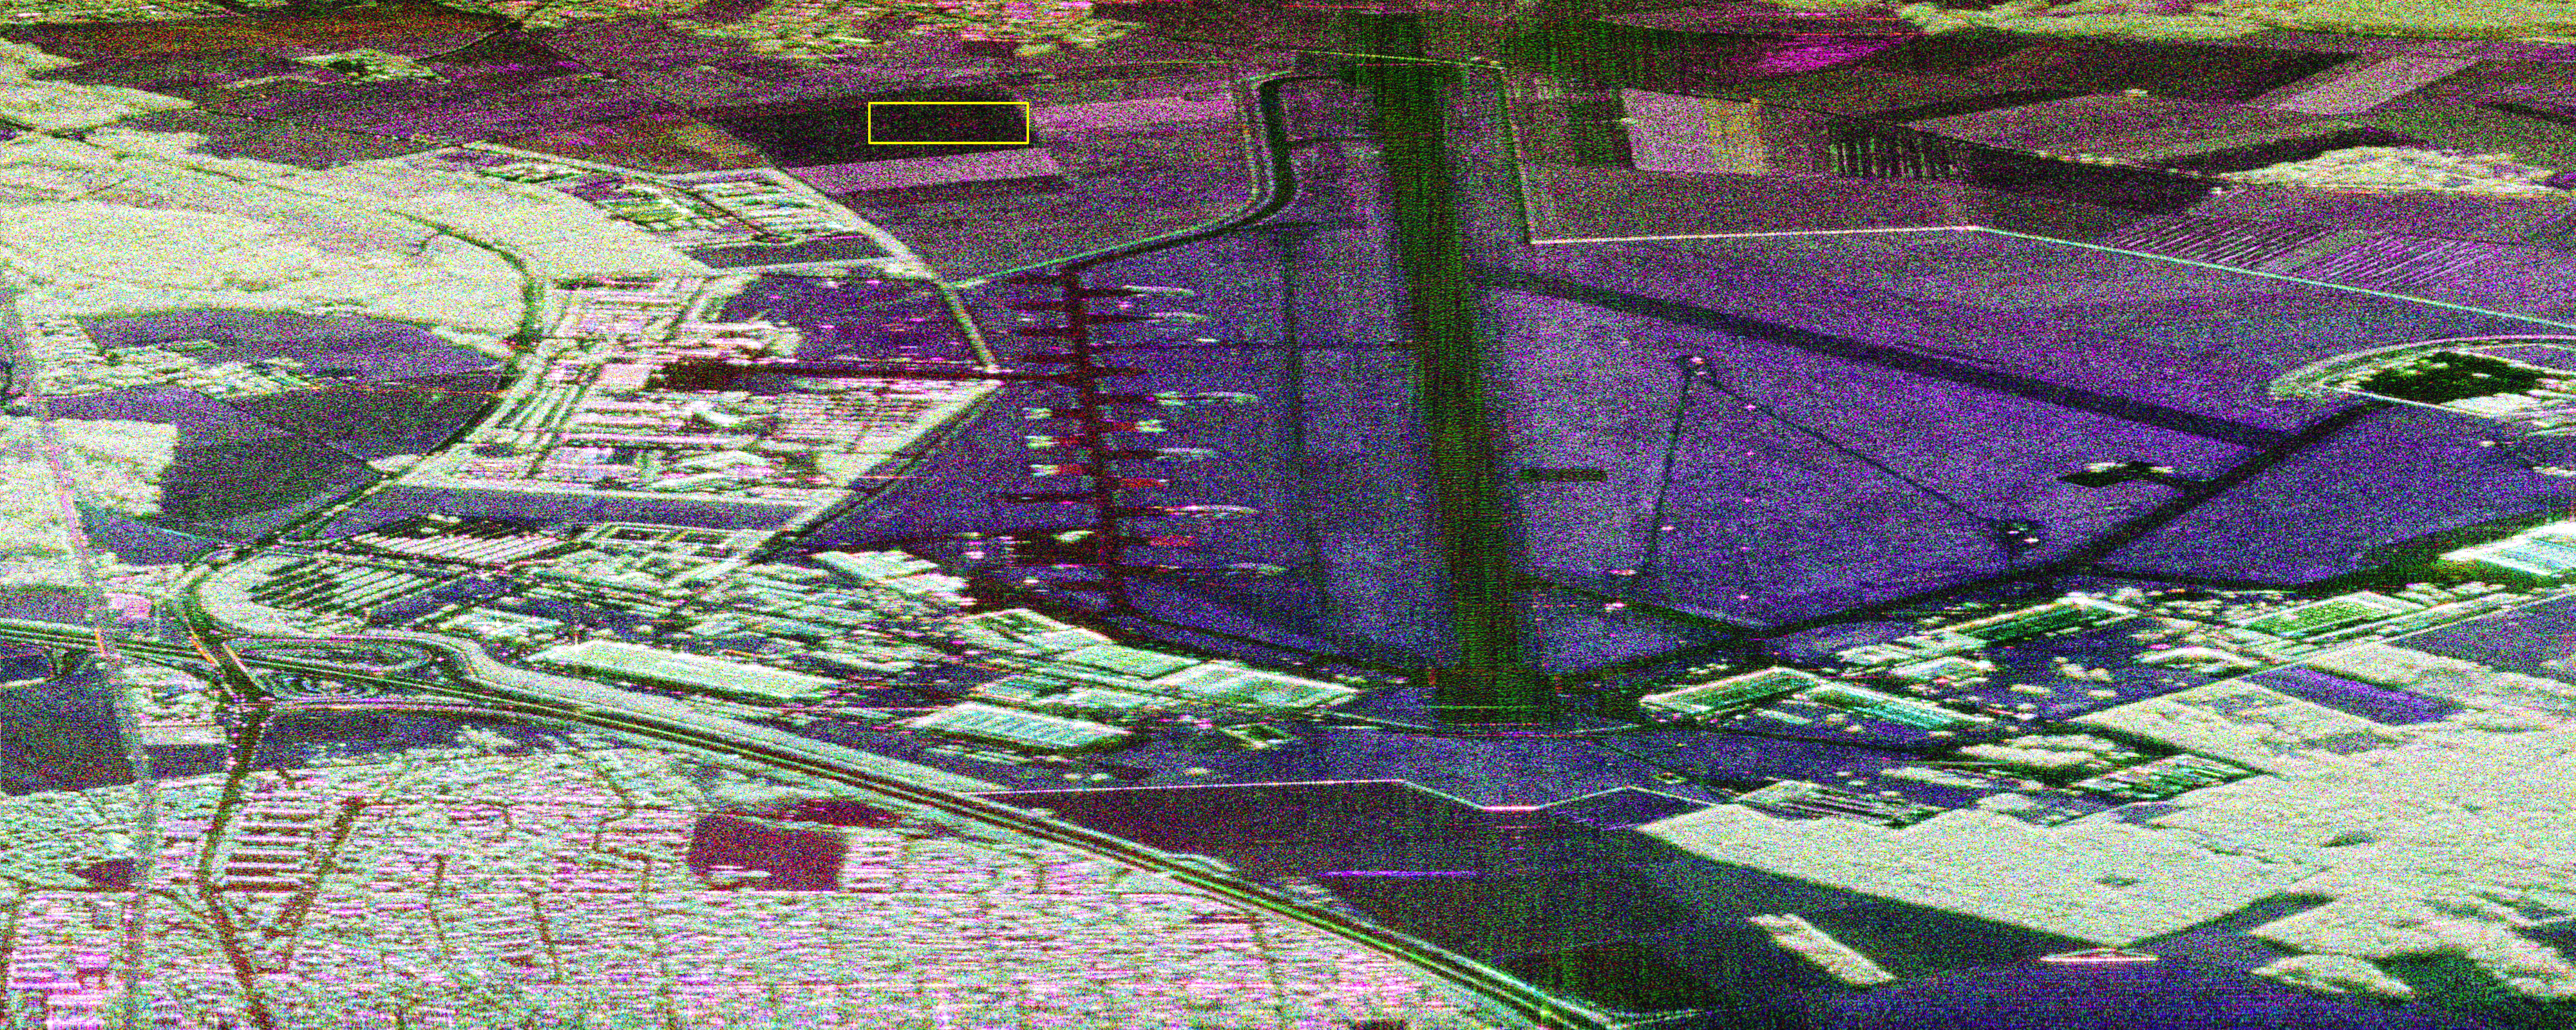
\includegraphics[width=\linewidth]{ESAR_RGB_Annot}
\caption{Color composition of the equalized intensity bands of an ESAR image over Oberpfaffenhofen}\label{Im:Oberpfaffenhofen_RGB}
\end{figure}

The image shown in Fig.~\ref{Im:Oberpfaffenhofen_RGB} has $1599\times4000$ pixels.
We selected $15561$ positions within the dark area in the upper part of the image, and extracted the observations both in the complex and intensity channels (without equalization).
This area, which is shown as a yellow rectangle, was chosen because there is no visual clue of texture in it.

Fig.~\ref{Fig:FittedDarkRegion_Complex} shows the histograms and fitted Gaussian densities of the six data sets corresponding to the real and imaginary parts of each polarization.
Notice that there is no evidence of either skewness or lack/excess of dispersion with respect to the hypothesized model.

\begin{figure}
\centering
\includegraphics[width=.32\linewidth]{dark_HH_Re}
\includegraphics[width=.32\linewidth]{dark_HH_Im}
\includegraphics[width=.32\linewidth]{dark_HV_Re}
\includegraphics[width=.32\linewidth]{dark_HV_Im}
\includegraphics[width=.32\linewidth]{dark_VV_Re}
\includegraphics[width=.32\linewidth]{dark_VV_Im}
\caption{Histograms and fitted Gaussian densities over the dark region of Fig.~\ref{Im:Oberpfaffenhofen_RGB}}\label{Fig:FittedDarkRegion_Complex}
\end{figure}

Fig.~\ref{Fig:FittedDarkRegion} shows the histograms and fitted Exponential densities of these three data sets.

\begin{figure}
\centering
\includegraphics[width=.32\linewidth]{darkHHfit}
\includegraphics[width=.32\linewidth]{darkHVfit}
\includegraphics[width=.32\linewidth]{darkVVfit}
\caption{Histograms and fitted Exponential densities over the dark region of Fig.~\ref{Im:Oberpfaffenhofen_RGB}}\label{Fig:FittedDarkRegion}
\end{figure}

The quality of the fit is remarkable, in particular for such large number of observations.
This is an empirical indication that the model we are considering is adequate.
\end{frame}


\section{The Multiplicative Model}

\begin{frame}[allowframebreaks]
One of the most famous statistical aphorisms is due to Prof.~George Box:
\begin{quotation}
The most that can be expected from any model is that it can supply a useful approximation to reality:

\textbf{All models are wrong; some models are useful.}
\end{quotation}
In line with this idea, in this chapter we will discuss the most important and illuminating models for SAR data that generalize the one for textureless data.

The Multiplicative Model is just one of the infinitely many ways to build stochastic descriptions for SAR data.
Among its advantages we would like to mention that it can be considered an \textit{ab initio} model, and that it leads to expressive and tractable descriptions of the data.
\end{frame}

\begin{frame}[allowframebreaks]
Let us recall that the basic model for multilook intensity data is the $\Gamma(\sigma^2,L)$ law whose density is
\begin{equation}
f_Z(z;L,\sigma^2) = \frac{L^L}{\sigma^{2L}\Gamma(L)} z^{L-1} 
	\exp\big\{ -L z / \sigma^2
	\big\}.
\end{equation}
As previously said, the Gamma distribution is scale-invariant, so we may pose this model as the product between the constant backscatter $X=\sigma^2$ and the multilook speckle $Y\sim\Gamma(1,L)$.

But, are there situations were we cannot assume a constant backscatter?
Yes, there are.
\end{frame}


\begin{frame}[allowframebreaks]
A constant backscatter results from infinitely many elementary backscatterers, i.e.\ from the assumption that $N\to\infty$ in~\eqref{Eq:ComplexBackscatter} (page~\pageref{Eq:ComplexBackscatter}).
Such assumption makes the particular choice of the sensed area irrelevant.
But this may not be the case always.

The advent of higher resolution sensors makes this hypothesis unsuitable in areas where the elementary backscatterers are of the order of the wavelength.
If, for instance, we are dealing with a \SI{1x1}{\meter} resolution image, we may consider $N\to\infty$ if the target is flat and composed of grass;
but if the target is a forest, this assumption may be unrealistic.

\end{frame}

\section{The $\mathcal K$ distribution}

\begin{frame}[allowframebreaks]

Assuming that the number of elementary backscatterers $N$ fluctuates according to a Negative Binomial distribution, one can obtain a closed-form density which characterizes the $\mathcal K$ distribution:
\begin{equation}
f_Z(z;\alpha,\lambda,L) =
\frac{2\lambda L}{\Gamma(\alpha)\Gamma(L)} (\lambda L z)^{\frac{\alpha+L}{2}-1} K_{\alpha-L}(2\sqrt{\lambda L z}),
\label{Eq:DensKI}
\end{equation}
where $\alpha>0$ measures the roughness, $\lambda>0$ is a scale parameter, and $K_\nu$ is the modified Bessel function of order $\nu$.
This special function is given by $K_\nu (z) = \int_0^\infty e^{-z} \cosh (\nu t) dt$.
This function is implemented in many numerical platforms as, for instance, in \texttt R.
\end{frame}

\begin{frame}[allowframebreaks]
We denote $Z\sim \mathcal K(\alpha,\lambda,L)$ the situation of $Z$ following the distribution characterized by~\eqref{Eq:DensKI}.
The $k$-order moments of $Z$ are
\begin{equation}
E(Z^k) = (\lambda L)^{-k} \frac{\Gamma(L+k)\Gamma(\alpha+k)}{\Gamma(L)\Gamma(\alpha)}.
\label{Eq:MomentKI}
\end{equation}
Eq.~\eqref{Eq:MomentKI} is useful, among other applications, for finding $\lambda^*=\alpha$, the scale parameter that yields a unitary mean distribution for each $\alpha$ and any $L$.
\end{frame}

\begin{frame}
Fig.~\ref{Fig:KIDistribution} shows the densities in linear and semilogarithmic scales of the Exponential and $\mathcal K$ distributions.
They all have unitary mean, and the latter is shown with different degrees of roughness ($\alpha\in\{1,3,8\}$).
It is noticeable that the larger the value of $\alpha$ is, the closer the $\mathcal K$ and $\text{E}$ densities become.
In fact, there is convergence in distribution of the latter to the former.
\end{frame}

\begin{frame}
\begin{figure}[hbt]
\centering
\subfloat[Densities]{\includegraphics[width=.48\linewidth]{KIDensities}}
\subfloat[Densities in semilog scale\label{Fig:DensKISemilog}]{\includegraphics[width=.48\linewidth]{KIDensitiesSemilog}}
\caption[Densities in linear and semilogarithmic scale of the $\text{E}(1)$ (green) and $\mathcal K$ distributions]{Densities in linear and semilogarithmic scale of the $\text{E}(1)$ (green) and $\mathcal K$ distributions with unitary mean ($\alpha\in\{1,3,8\}$ in red, blue, and black, resp.)}\label{Fig:KIDistribution}
\end{figure}
\end{frame}

\begin{frame}
The difference between these distributions is noteworthy, c.f.\ Fig.~\ref{Fig:KIDistribution}\subref{Fig:DensKISemilog}.
The green straight line is the density of the Exponential distribution, while the red one is that of the $\mathcal K(1,1,1)$ law.
The latter assigns larger probabilities to both small and large values, when compared with the former.
This leads, as will be seen later, to very contrasted data.

Fig.~\ref{Fig:KIDistributionLooks} shows the effect of varying the number of looks, for the same $\alpha=2$ and $\lambda=2$.
\end{frame}

\begin{frame}
\begin{figure}[hbt]
\centering
\subfloat[Densities]{\includegraphics[width=.48\linewidth]{KIDensitiesLooks}}
\subfloat[Densities in semilog scale\label{KIDensitiesSemilog}]{\includegraphics[width=.48\linewidth]{KIDensitiesSemilogLooks}}
\caption[Densities in linear and semilogarithmic scale $\mathcal K(2,2,L)$ distributions with unitary mean and $L\in\{1,3,8\}$]{Densities in linear and semilogarithmic scale $\mathcal K(2,2,L)$ distributions with unitary mean and $L\in\{1,3,8\}$ in red, blue, and black, resp.)}\label{Fig:KIDistributionLooks}
\end{figure}
\end{frame}

\begin{frame}
Notice in Fig~\ref{Fig:KIDistributionLooks}\subref{KIDensitiesSemilog} the dramatic effect multilook processing has mostly on the distribution of very small values.
This, along with the reduced probability very large values have with multilook processing, yields less contrasted images.

Although the basic construction, and physical explanation, of the $\mathcal K$ distribution stems from letting fluctuate the number of elementary backscatters, we are interested in an equivalent derivation.
\end{frame}

\begin{frame}
As previously said, the basic model for observations without roughness is~\eqref{eq:SARGammaDensity}.
The mean $X=\sigma^2$ can be seen as multiplying $Y$, a $\Gamma(1,L)$ random variable, which describes the speckle.
As we are interested in letting the mean fluctuate, $X$ can be described by any distribution with positive support.
If we choose a Gamma random variable with mean $\alpha/\lambda>0$ and shape parameter $\alpha>0$, i.e., $Y\sim\Gamma(\alpha/\lambda,\alpha)$, and further assume that $X$ and $Y$ are independent, then the product $Z=XY$ follows a $\mathcal{K}(\alpha,\lambda,L)$ distribution with density~\eqref{Eq:DensKI}.
This \textit{multiplicative} construction is not only useful for sampling from this distribution, but also for obtaining other models for the return.
\end{frame}


\section{The $\mathcal G^0$ distribution}

\begin{frame}
The $\mathcal{K}$ distribution fails at describing data from extremely textured areas as, for instance, urban targets.
The authors then proposed a different model for the backscatter $X$: the Reciprocal Gamma distribution.

We say that $X\sim{\Gamma^{-1}}(\alpha,\gamma)$, with $\alpha<0$ and $\gamma>0$ follows a 
Reciprocal Gamma distribution is characterized by the density
\begin{equation}
f_X(x;\alpha,\gamma) = \frac{1}{\gamma^\alpha} x^{\alpha-1} \exp\{-\gamma/x\},
\label{Eq:IGdensity}
\end{equation}
for $x>0$ and zero otherwise.
\end{frame}


\begin{frame}
Now introducing the Reciprocal Gamma model for the backscatter in the multiplicative model, i.e. by multiplying the independent random variables $X\sim{\Gamma^{-1}}(\alpha,\gamma)$ and $Y\sim\Gamma(1,L)$, one obtains the $\mathcal{G}^0$ distribution for the return $Z=XY$, which is characterized by the density
\begin{equation}
f_Z(z; \alpha,\gamma,L) = \frac{L^L \Gamma(L-\alpha)}{\gamma^\alpha \Gamma(L)\Gamma(-\alpha)} \frac{z^{L-1}}{(\gamma+L z)^{L-\alpha}},
\label{Eq:DensGI0}
\end{equation}
where $\alpha<0$, and $\gamma,z>0$.
It is noteworthy that, differently from~\eqref{Eq:DensKI}, this density does not involve Bessel functions.

We denote $Z\sim \mathcal G^0(\alpha,\gamma,L)$ the situation of $Z$ following the distribution characterized by~\eqref{Eq:DensGI0}.
The $k$-order moments of $Z$ are
\begin{equation}
E(Z^k) = (\gamma / L)^{k} \frac{\Gamma(L+k)\Gamma(-\alpha-k)}{\Gamma(L)\Gamma(-\alpha)},
\label{Eq:MomentGI0}
\end{equation}
provided $-\alpha>k$, and infinite otherwise.
Eq.~\eqref{Eq:MomentGI0} is useful, among other applications, for finding $\gamma^*=-\alpha-1$, the scale parameter that yields a unitary mean distribution for each $\alpha$ and any $L$.
\end{frame}


\begin{frame}
Fig.~\ref{Fig:GI0Distribution} shows the $\text{E}(1)$ and $\mathcal G^0(\alpha,\gamma^*, 1)$ densities.
The differences in tail behavior are clearly exhibited in the semilogarithmic scale; cf.\ Fig.~\ref{Fig:GI0Distribution}\subref{Fig:DensGI0Semilog}.
Whereas the exponential distribution decreases linearly, the $\mathcal G^0$ law assigns more probability to larger events increasing, thus, the variability of the return.
\end{frame}


\begin{frame}
\begin{figure}[hbt]
\centering
\subfloat[Densities]{\includegraphics[width=.48\linewidth]{GI0Densities}}
\subfloat[Densities in semilog scale\label{Fig:DensGI0Semilog}]{\includegraphics[width=.48\linewidth]{GI0DensitiesSemilog}}
\caption[Densities in linear and semilogarithmic scale of the $\text{E}(1)$ (green) and $\mathcal G^0$ distributions with unitary mean]{Densities in linear and semilogarithmic scale of the $\text{E}(1)$ (green) and $\mathcal G^0$ distributions with unitary mean and $\alpha\in\{-1.5,-3,-8\}$ in red, blue, and black, resp.}\label{Fig:GI0Distribution}
\end{figure}
\end{frame}


\begin{frame}
Fig.~\ref{Fig:GI0DistributionLooks} shows the effect of varying the number of looks, for the same $\alpha=5$ and $\gamma=4$.

Notice, again, in Fig~\ref{Fig:GI0DistributionLooks}\subref{GI0DensitiesSemilog} the effect multilook processing has mostly on the distribution of very small values.
This, along with the reduced probability very large values have with multilook processing, yields less contrasted images.
\end{frame}


\begin{frame}
\begin{figure}[hbt]
\centering
\subfloat[Densities]{\includegraphics[width=.48\linewidth]{GI0DensitiesLooks}}
\subfloat[Densities in semilog scale\label{GI0DensitiesSemilog}]{\includegraphics[width=.48\linewidth]{GI0DensitiesSemilogLooks}}
\caption[Densities in linear and semilogarithmic scale $\mathcal G^0(-5,4,L)$ distributions with unitary mean and $L\in\{1,3,8\}$]{Densities in linear and semilogarithmic scale $\mathcal G^0(-5,4,L)$ distributions with unitary mean and $L\in\{1,3,8\}$ in red, blue, and black, resp.)}\label{Fig:GI0DistributionLooks}
\end{figure}
\end{frame}


\begin{frame}
The $\mathcal{G}^0$ distribution has the same number of parameters as the $\mathcal{K}$ law, but it has been shown to be more apt at modeling return with extreme variability.
Moreover, it is also able to describe the same kind of return from textured areas for which the latter was proposed.
It has been shown that, with proper choices of parameters, the $\mathcal G^0$ law can approximate with any error any $\mathcal K$ distribution.
For these reasons, the $\mathcal G^0$ distribution is called \textit{``Universal Model''} for SAR data.
\end{frame}

\begin{frame}
The $\mathcal G^0$ distribution relates to the well-known Fisher-Snedekor law in the following manner:
\begin{equation}
F_{G^0(\alpha,\gamma,L)}(t) = \Upsilon_{2L,- 2\alpha}(- \alpha t/\gamma),
\end{equation}
where $\Upsilon_{u,v}$ is the cumulative distribution function of a Fisher-Snedekor distribution with $u$ and $v$ degrees of freedom, and $F_{G^0(\alpha,\gamma,L)}$ is the cumulative distribution function of a $F_{G^0(\alpha,\gamma,L)}$ random variable.
Notice that $\Upsilon$ is readily available in most software platforms for statistical computing.
Since such platforms usually also provide implementations of the inverse of cumulative distribution functions, the Inversion Theorem can be used to sample from the $\mathcal G^0$ law.
\end{frame}

\begin{frame}
Arguably, the most popular way of sampling from the $\mathcal G^0$ distribution is through its multiplicative nature.
Obtaining deviates from $X\sim\Gamma(1,L)$ is immediate.
In order to sample from $Y\sim\Gamma^{-1}(\alpha,\gamma)$, one may use the fact that if $Y'\sim\Gamma(-\alpha,\gamma)$, then $Y=1/Y'$ has $\Gamma^{-1}(\alpha,\gamma)$ distribution.
Then, $Z=X/Y'$ has the desired $\mathcal G^0(\alpha,\gamma,L)$ distribution.
\end{frame}

\begin{frame}{Final Recommendations}
\begin{itemize}
\item The statistical properties of SAR data carry lots of information.
\item This information is valuable for many applications: classification, segmentation, speckle reduction, processing and understanding.
\item You do not have to be a statistician to take advantage of this information.
\item An operational viewpoint requires a good statistical culture, and tools.
\item Work driven by your questions, rather than by the answers you already have.
\end{itemize}
\end{frame}

\section{Starting with R}

\begin{frame}{Why R?}
	\begin{itemize}
		\item Multiplatform
		\item Interplatform
		\item Numerically dependable
		\item Thousands of libraries
		\item Active and supportive community
		\item Promotes reproducibility
		\item It is free
	\end{itemize}
\end{frame}

\begin{frame}{Resources}
	\begin{itemize}
		\item \url{http://www.r-project.org}
		\item \url{http://	www.rstudio.com}
		\item \url{https://ggplot2.tidyverse.org/}
		\item \url{http://www.ggplot2-exts.org/gallery/}
	\end{itemize}
	
\end{frame}

\end{document}

